\subsubsection{Package com.sirius.sequenziatore.server.presenter.processowner}
\begin{figure}[H] \centering 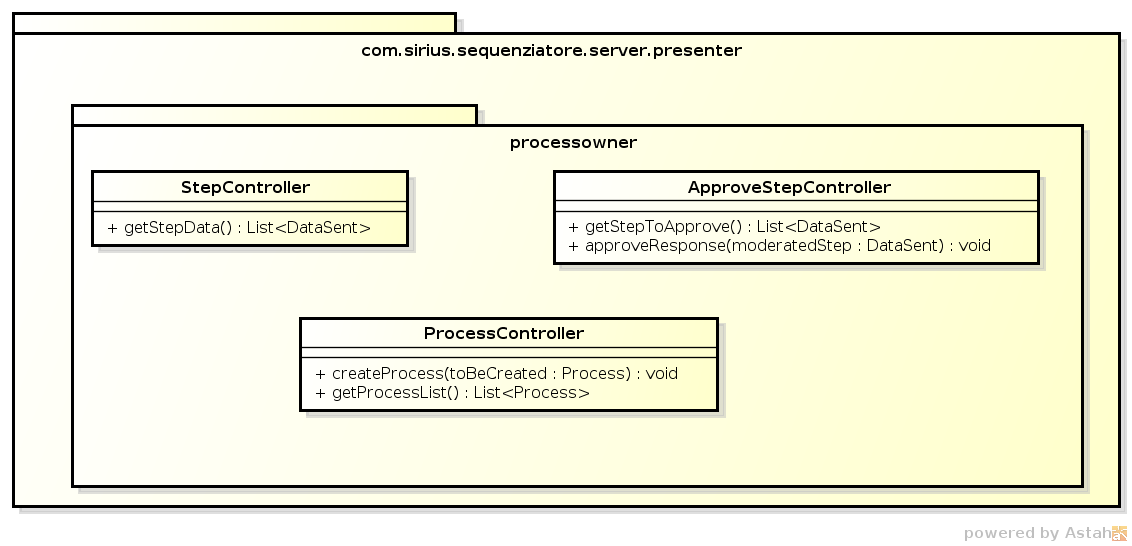
\includegraphics[width=%
\textwidth]
{./classi/server/presenterprocessowner.png} \caption{Diagramma package - \texttt{com.sirius.sequenziatore.server.presenter.processowner}}
\end{figure}
\paragraph{StepController}%----------------------------------------------------------------%
\
\begin{figure}[H] \centering
\includegraphics[trim=0cm 0.8cm 0cm 0cm,clip=true,scale=0.75]%
{./classi/server/stepcontroller.png} \caption{Diagramma classe - \texttt{StepController}}
\end{figure}
\begin{itemize}
	\item \textbf{Descrizione: } Questa classe dovrà fornire al \textit{process owner} tutti i dati inseriti dagli utenti per un dato passo, quindi dovrà restituire una collezione di dati al process owner il quale potrà visionarli;
	\item \textbf{Mappatura base: } \textit{\textbackslash stepdata\textbackslash \{idstep\}\textbackslash processowner}
	\item \textbf{Relazioni con altri componenti: }
	La classe utilizzerà le seguenti classi:
	\begin{itemize}
		\item \texttt{com.sirius.sequenziatore.server.model.DataSent;}
		\item \texttt{com.sirius.sequenziatore.server.model.StepDao;}
	\end{itemize}
	tramite le interfacce:
	\begin{itemize}
		\item \texttt{com.sirius.sequenziatore.server.model.ITransferObject;}
		\item \texttt{\sModel .IDataAccessObject;}
	\end{itemize}
	\item \textbf{Metodi: }\begin{itemize}
					\item \texttt{+List<StepData> getStepData():}\\
					questo metodo gestisce una richiesta di tipo \textbf{GET} che fornisce al \textit{process owner} tutti i dati inviati dagli utenti per un certo passo;
				\end{itemize}
\end{itemize}
\paragraph{ProcessController}%----------------------------------------------------------------%
\
\begin{figure}[H] \centering
\includegraphics[trim=0cm 0.8cm 0cm 0cm,clip=true,scale=0.75]%
{./classi/server/processcontroller.png} \caption{Diagramma classe - \texttt{ProcessController}}
\end{figure}
\begin{itemize}
	\item \textbf{Descrizione: } Questa classe permetterà la creazione di un processo da parte del \textit{process owner} e sarà adibita a fornire la lista di tutti i processi esistenti nel sistema;
	\item \textbf{Mappatura base: } \textit{\textbackslash process\textbackslash processowner}
	\item \textbf{Relazioni con altri componenti: }
	La classe utilizzerà le seguenti classi:
	\begin{itemize}
		\item \texttt{com.sirius.sequenziatore.server.model.Process;}
		\item \texttt{com.sirius.sequenziatore.server.model.ProcessDao;}
	\end{itemize}
	tramite le interfacce:
	\begin{itemize}
		\item \texttt{com.sirius.sequenziatore.server.model.ITransferObject;}
		\item \texttt{\sModel .IDataAccessObject;}
	\end{itemize}
	\item \textbf{Metodi: }
				\begin{itemize}
					\item \texttt{+void createProcess(Process toBeCreated):}\\
					questo metodo gestisce una richiesta di tipo \textbf{POST} e permette l' inserimento del processo fornito nel \textit{database};
					\item \texttt{+List<Process> getProcessList():}\\
					 questo metodo gestisce una richiesta di tipo \textbf{GET} e restituisce al \textit{process owner} una lista di processi che può visualizzare;
				\end{itemize}
\end{itemize}
\paragraph{ApproveStepController}%----------------------------------------------------------------%
\
\begin{figure}[H] \centering
\includegraphics[trim=0cm 0.8cm 0cm 0cm,clip=true,scale=0.75]%
{./classi/server/approvestepcontroller.png} \caption{Diagramma classe - \texttt{ApproveStepController}}
\end{figure}
\begin{itemize}
	\item \textbf{Descrizione: } Questa classe serve per fornire al \textit{process owner} i dati da approvare e per gestire quali passi siano stati approvati quali no, qualora un passo non venga approvato, verrà rimosso dal \textit{database};
	\item \textbf{Mappatura base: } \textit{\textbackslash approvedata}
	\item \textbf{Relazioni con altri componenti: }
	La classe utilizzerà le seguenti classi:
	\begin{itemize}
		\item \texttt{com.sirius.sequenziatore.server.model.DataSent;}
		\item \texttt{com.sirius.sequenziatore.server.model.StepDao;}
	\end{itemize}
	tramite le interfacce:
	\begin{itemize}
		\item \texttt{com.sirius.sequenziatore.server.model.ITransferObject;}
		\item \texttt{\sModel .IDataAccessObject;}
	\end{itemize}
	\item \textbf{Metodi: }\begin{itemize}
					\item \texttt{+List<DataSent> getStepToApprove():}\\
					 il metodo gestisce una richiesta di tipo \textit{GET}, e restituirà un oggetto di tipo List<DataSent> contenente tutti i dati che richiedono approvazione;
					\item \texttt{+void approveResponse(int idStep,String usernameww):}\\
					il metodo gestisce una richiesta di tipo \textit{POST}, riceve i dati di un passo che ha subito la moderazione del \textit{process owner}, tale passo verrà eliminato dal database se il processowner lo ha rifiutato altrimenti verrà approvato definitivamente;  
				\end{itemize}
\end{itemize}